\documentclass[12pt,]{article}
\usepackage{lmodern}
\usepackage{amssymb,amsmath}
\usepackage{ifxetex,ifluatex}
\usepackage{fixltx2e} % provides \textsubscript
\ifnum 0\ifxetex 1\fi\ifluatex 1\fi=0 % if pdftex
  \usepackage[T1]{fontenc}
  \usepackage[utf8]{inputenc}
\else % if luatex or xelatex
  \ifxetex
    \usepackage{mathspec}
    \usepackage{xltxtra,xunicode}
  \else
    \usepackage{fontspec}
  \fi
  \defaultfontfeatures{Mapping=tex-text,Scale=MatchLowercase}
  \newcommand{\euro}{€}
\fi
% use upquote if available, for straight quotes in verbatim environments
\IfFileExists{upquote.sty}{\usepackage{upquote}}{}
% use microtype if available
\IfFileExists{microtype.sty}{%
\usepackage{microtype}
\UseMicrotypeSet[protrusion]{basicmath} % disable protrusion for tt fonts
}{}
\usepackage[margin=1in]{geometry}
\usepackage{graphicx}
\makeatletter
\def\maxwidth{\ifdim\Gin@nat@width>\linewidth\linewidth\else\Gin@nat@width\fi}
\def\maxheight{\ifdim\Gin@nat@height>\textheight\textheight\else\Gin@nat@height\fi}
\makeatother
% Scale images if necessary, so that they will not overflow the page
% margins by default, and it is still possible to overwrite the defaults
% using explicit options in \includegraphics[width, height, ...]{}
\setkeys{Gin}{width=\maxwidth,height=\maxheight,keepaspectratio}
\ifxetex
  \usepackage[setpagesize=false, % page size defined by xetex
              unicode=false, % unicode breaks when used with xetex
              xetex]{hyperref}
\else
  \usepackage[unicode=true]{hyperref}
\fi
\hypersetup{breaklinks=true,
            bookmarks=true,
            pdfauthor={},
            pdftitle={},
            colorlinks=true,
            citecolor=blue,
            urlcolor=black,
            linkcolor=black,
            pdfborder={0 0 0}}
\urlstyle{same}  % don't use monospace font for urls
\setlength{\parindent}{0pt}
\setlength{\parskip}{6pt plus 2pt minus 1pt}
\setlength{\emergencystretch}{3em}  % prevent overfull lines
\setcounter{secnumdepth}{0}

%%% Use protect on footnotes to avoid problems with footnotes in titles
\let\rmarkdownfootnote\footnote%
\def\footnote{\protect\rmarkdownfootnote}

%%% Change title format to be more compact
\usepackage{titling}

% Create subtitle command for use in maketitle
\newcommand{\subtitle}[1]{
  \posttitle{
    \begin{center}\large#1\end{center}
    }
}

\setlength{\droptitle}{-2em}
  \title{}
  \pretitle{\vspace{\droptitle}}
  \posttitle{}
  \author{}
  \preauthor{}\postauthor{}
  \date{}
  \predate{}\postdate{}

\usepackage{lineno}
\linenumbers
\usepackage{setspace}
\usepackage{todonotes}
\doublespacing
\usepackage{rotating}
\usepackage{color, soul}
\usepackage[font={footnotesize},labelfont={sf,bf},labelsep=space]{caption}
\usepackage{sectsty}


\begin{document}

\maketitle


\renewcommand\linenumberfont{\normalfont\tiny\sffamily\color{gray}}

\begin{singlespace}

\begin{centering}

\Large{How fluctuation-dependent species coexistence affects the diversity-stability relationship}



\vspace{2.5em}

\renewcommand*{\thefootnote}{\fnsymbol{footnote}}

\normalsize{Andrew T. Tredennick\textsuperscript{1}, Peter B. Adler\textsuperscript{1}, and Frederick R. Adler\textsuperscript{2}}

\vspace{1.5em}

\textit{\small{\textsuperscript{1}Department of Wildland Resources and the Ecology Center, Utah State University, Logan, Utah 84322}} \\
\textit{\small{\textsuperscript{2}Departments of Biology and Mathematics, University of Utah, Salt Lake City, Utah}} 

\end{centering}

\vspace{3em}

\noindent \textbf{Keywords}: coexistence, storage effect, relative nonlinearity, diversity-stability hypothesis, pulsed differential equation, consumer-resource dynamics

\noindent \textbf{Authorship}: All authors conceived the research and designed the modeling approach; ATT conducted model simulations, with input from PBA and FRA; ATT wrote the manuscript and all authors contributed to revisions.

\noindent \textbf{Running Title}: Environmental variability, ecosystem stability, \& species coexistence

\noindent \textbf{Article Type}: Letter

\noindent \textbf{Number of Words}:

\noindent \textbf{Number of References}:

\noindent \textbf{Number of Tables and Figures}:

\noindent \textbf{Corresponding Author}:  \\
Andrew Tredennick  \\
Department of Wildland Resources and the Ecology Center  \\
Utah State University  \\
5230 Old Main Hill  \\
Logan, Utah 84322 USA  \\
Phone: +1-970-443-1599  \\
Fax: +1-435-797-3796  \\
Email: atredenn@gmail.com

\end{singlespace}

\newpage{}

\begin{abstract}
Theory relating species richness to ecosystem stability typically ignores the potential for environmental variability to promote species coexistence.
Failure to account for fluctuation-dependent coexistence mechanisms may explain observed deviations from the expected positive diversity-stability relationship, and limits our ability to predict the consequences of increasing environmental variability.
We use a consumer-resource model to explore how coexistence via the temporal storage effect and relative nonlinearity affects ecosystem stability.
We show that a negative, rather than positive, diversity-stability relationship is possible when ecosystem function is sampled across a natural gradient in environmental variability and diversity.
We also show how fluctuation-dependent coexistence can buffer ecosystem functioning against increasing environmental variability by allowing more species to coexist and contribute to portfolio effects.
Our work provides a general explanation for variation in observed diversity-stability relalationships and highlights the importance of conserving regional species pools to help buffer ecosystems against future increases in environmental variability.
\vspace{2em}
\end{abstract}

\newpage{}

\setlength{\parindent}{5ex}

\subsection{INTRODUCTION}\label{introduction}

MacArthur (1955), Elton (1958), and even Darwin (Turnbull et al. 2013)
recognized that species can compensate for each other and stabilize
ecosystem functioning in fluctuating environments. This idea underlies
the ``insurance hypothesis'' (Yachi and Loreau 1999), which suggests
stability increases with diversity because species respond dissimilarly
to environmental conditions, broadening the range of conditions under
which the community maintains function (Loreau 2010). Diverse models all
predict a positive relationship between species richness and ecosystem
stability (Lehman and Tilman 2000, Ives and Hughes 2002, Loreau and {{de
Mazancourt}} 2013), and experimental tests tend to support such a
prediction (Tilman et al. 2006, Hector et al. 2010).

However, the ability of biodiversity-ecosystem functioning (BEF)
experiments to represent real-world dynamics is the subject of debate
(Wardle 2016, Eisenhauer et al. 2016). Much of the debate centers around
the fact that species losses in BEF experiments are not allowed to be
offset by species gains. Theoretical work on diveristy-stability
relationships typically suffers from the same limitation, ignoring the
processes by which temporal environmental variability can promote
coexistence and increase species richness (Loreau 2010, but see Chesson
et al. 2001).

Fluctuating environmental conditions are an important ingredient for
stable species coexistence, both in theoretical models (Chesson 2000a,
Chesson et al. 2004) and in natural communities (C{á}ceres 1997,
Descamps-Julien and Gonzalez 2005, Adler et al. 2006, Angert et al.
2009). Such ``fluctuation-dependent'' coexistence requires that species
have unique environmental responses and that environmental conditions
vary so that each species in a community experiences favorable and
unfavorable conditions, which prevents competitive exclusion (Chesson
2000a). When coexistence is maintained by a fluctuation-dependent
mechanism, an increase in environmental variability might lead to an
increase in species richness and, consequently, an increase in ecosystem
stability. However, increasing environmental variability may also
decrease ecosystem stability by increasing the fluctuations of
individual species, regardless of species richness.

The countervailing effects of environmental variability present an
interesting paradox: increasing variability should decrease ecosystem
stability, but the potential for an increase in richness might offset
the decrease in stability. Such a paradox complicates predictions about
how ecosystems will respond as environmental conditions exceed
historical ranges of variability. The unknown net effect of environment
variability may be reflected in the mixed results from empirical studies
on the diversity-stability relationship. Observational tests of the
diversity-stability relationship, which require sampling across natural
diversity gradients, have yielded positive (Hautier et al. 2014),
neutral (Valone and Hoffman 2003, Cusson et al. 2015), and negative
(Sasaki and Lauenroth 2011) relationships. In a meta-analysis of
diversity-stability relationships based on observational studies in
terrestrial ecosystems, Jiang and Pu (2009) found no significant
evidence for an effect of species richness on ecosystem stability. The
idiosyncratic results of these empirical studies contrasts with the
consistent conclusions from theoretical work.

The gap between theoretical expectations and empirical results of
richness-stability relationships reflects the divergence of theory
developed to explain species coexistence and theory developed to explain
diversity and stability. One reason these two disciplines have diverged
is because they have focused on slightly different questions.
Diversity-stability studies typically ask how ecosystem variability
responds to different levels of species richness at a given level of
environmental variability (reviewed in Kinzig et al. 2001, Loreau 2010),
whereas coexistence studies ask how the long term stability of species
coexistence responds to different levels of environmental variability
(Chesson and Warner 1981).

To reconcile these two perspectives, we extend theory on the
relationship between species richness and ecosystem stability to cases
in which species coexistence explicitly depends on environmental
fluctuations and species-specific responses to environmental conditions.
We focus on the temporal storage effect and relative nonlinearity using
a general consumer-resource model. We use the model to investigate three
questions:

\begin{enumerate}
\def\labelenumi{\arabic{enumi}.}
\item
  Does the direction of the diversity-stability relationship remain
  positive when species coexistence is fluctuation-dependent?
\item
  When species coexistence is fluctuation-dependent, how does increasing
  environmental variability impact ecosystem stability?
\item
  Do our answers to the previous two questions depend on the specific
  fluctuation-dependent coexistence mechanism (i.e., storage effect
  vs.~relative nonlinearity)?
\end{enumerate}

\subsection{MATERIALS AND METHODS}\label{materials-and-methods}

\subsubsection{Consumer-resource model}\label{consumer-resource-model}

We developed a semi-discrete consumer-resource model that allows many
species to coexist on one resource by either the storage effect or
relative nonlinearity. In our model, the consumer can be in one of
two-states: a dormant state \(D\) and a live state \(N\). The dormant
state could represent, for example, the seedbank of an annual plant.
Transitions between \(N\) and \(D\) occur at discrete intervals \(\tau\)
with continuous-time consumer-resource dynamics between discrete
transitions. Thus, our model is formulated as ``pulsed differential
equations'' (Pachepsky et al. 2008, Mailleret and Lemesle 2009, Mordecai
et al. 2016). For clarity we refer to \(\tau\) as years and the growing
time between years as seasons with daily (\(t\)) time steps.

During a growing season, consumer-resource dynamics are modeled as two
differential equations:

\begin{align}
\frac{\text{d}N_{i}}{\text{d}t} &= N_{i}\epsilon_if_{i}(R), \quad t \ne \tau_k\\
\frac{\text{d}R}{\text{d}t} &= - \sum\limits_{i=1,2}f_{i}(R)N_{i}, \quad t \ne \tau_k
\end{align}

\noindent where the discrete transitions between \(N\) and \(D\) occur
between seasons at times \(\tau_k\), \(k = 1,2,3, \dots, K\). The
subscript \(i\) denotes species, \(N\) is the living biomass state, and
\(\epsilon_i\) is each species' resource-to-biomass conversion
efficiency. The growth rate of living biomass is a resource-dependent
Hill function,
\(f_{i}(R) = r_{i}R^{a_{i}} / (b_{i}^{a_{i}}+R^{a_{i}})\), where
\emph{r} is a species' intrinsic growth rate and \emph{a} and \emph{b}
define the curvature of the function. Resource depletion is equal to the
sum of each species' consumption.

Along with resource uptake, consumer population growth depends on the
production of dormant biomass (\(D\)), the activation of dormant biomass
to live biomass (\(D \rightarrow N\)), and the survival of living
biomass from one year to the next. The biomass of each species' states
at the start of a growing season are equal to

\begin{align}
  D_{i}(\tau_k^+) &= (1-\gamma_{i,\tau_k})[\alpha_i N_{i}(\tau_k) + D_{i}(\tau_k)](1-\eta_i) \\
  N_{i}(\tau_k^+) &= (1-\alpha_i)N_{i}(\tau_k) + \gamma_{i,t}[\alpha_i N_{i}(\tau_k) + D_{i}(\tau_k)] (1-\eta_i),
\end{align}

\noindent where \(D(\tau_k)\), \(N(\tau_k)\), and \(R(\tau_k)\) are the
abundances of each state at the end of growing season \emph{k} and
\(\tau_k^+\) denotes the beginning of growing season \(k=1\). The
activation of dormant biomass to live biomass is controlled by
\(\gamma\), which is year (\emph{k}) and species (\emph{i}) specific.
Dormant biomass is equal to a constant fraction (\(\alpha\)) of live
biomass at the end of the previous season (\(N_{i}(\tau_k)\)), plus
survival (\(1-\eta_i\)) of dormant biomass (\(D_{i}(\tau_k)\)) at the
end of the previous year and dormant biomass remaining after live
biomass activation (\(D_{i}(\tau_k)(1-\gamma_{i,\tau_k})\)). Live
biomass is equal to newly activated dormant biomass
(\(\gamma_{i,t}[D_{i}(\tau_k)\)), minus some fraction of live biomass
that is converted to dormant biomass (\((1-\alpha_i)N_{i}(\tau_k)\)) We
assume the resource pool is not replenished within a growing season.
Resource replenishment occurs between growing seasons, and the resource
pool (\emph{R}) at the start of the growing season \emph{k}+1 is
\(R(\tau_k^+) = R^+\), where \(R^+\) is a random resource pulse drawn
from a log-normal distribution with mean \(\mu(R^+)\) and standard
deviation \(\sigma(R^+)\). Model parameters and notation are described
in Table 1.

\paragraph{Implementing the Storage
Effect}\label{implementing-the-storage-effect}

For the storage effect to operate, we need species-specific responses to
environmental variability, density-dependent covariance between
environmental conditions and competition (\emph{EC} covariance), and
subadditive population growth (Chesson 1994, 2000b). Regardless of the
mechanism, long-term coexistence is possible when all species can
increase when rare. In the storage effect, rare species increase by
escaping the effects of \emph{EC} covariance. This happens because
common species will experience greater than average competition
(\emph{C}) in good environment (\emph{E}) years because common species
cannot avoid intraspecific competition. Rare species do not have this
problem and can increase rapdily in a good \emph{E} year. \emph{EC}
covariance is included in our model because dormant-to-live transition
rates (\(\gamma\)) are species-specific and vary through time. In a high
\(\gamma\) year for a common species, resource uptake will be above
average, while in a high \(\gamma\) year for a rare species, resource
uptake will be below average.

Subadditive population growth buffers populations against large
population decreases in unfavorable years. It is included in our model
because we include a dormant stage with very low death rates, which
limits large population declines. In combination, subadditive population
growth limits population declines in bad \emph{E} years, and \emph{EC}
covariance ensures species can increase rapidly when rare but suffer
when common.

We generated sequences of (un)correlated dormant-to-live state
transition rates (\(\gamma\)) for each species by drawing from
multivariate normal distributions with mean 0 and a variance-covariance
matrix (\(\Sigma(\gamma)\)) of

\begin{align}
\Sigma(\gamma) = 
\begin{bmatrix}
\sigma^2_{E} & \rho_{1,2}\sigma^2_{E} & \rho_{1,3}\sigma^2_{E} & \rho_{1,4}\sigma^2_{E} \\
\rho_{2,1}\sigma^2_{E} & \sigma^2_{E} & \rho_{2,3}\sigma^2_{E} & \rho_{2,4}\sigma^2_{E} \\
\rho_{3,1}\sigma^2_{E} & \rho_{3,2}\sigma^2_{E} & \sigma^2_{E}  & \rho_{3,4}\sigma^2_{E} \\
\rho_{4,1}\sigma^2_{E} & \rho_{4,2}\sigma^2_{E} & \rho_{4,3}\sigma^2_{E} & \sigma^2_{E}  \\
\end{bmatrix}
\end{align}

\noindent where \(\sigma^2_{E}\) is the variance of the environmental
cue and \(\rho_{i,j}\) is the correlation between between the species
\emph{i}'s and species \emph{j}'s transition rates. \(\rho\) must be
less than 1 for stable coexistence, and in all simulations we placed
that constraint that \(\rho_{i,j} = \rho_{j,i}\) for each species pair.
The inferior competitor has the strongest potential to persist when
\(\rho=-1\) (perfectly uncorrelated transition rates). We used the
\texttt{R} function \texttt{mvrnorm} to generate sequences of
(un)correlated variates \emph{E} that we converted to germination rates
in the 0-1 range: \(\gamma = e^E / 1 + e^E\). Note that
\(\Sigma(\gamma)\) must be positive definite. So, after defining
\(\Sigma(\gamma)\) with all \(\rho_{i,j}\)s and \(\sigma^2_{E}\), we
used the \texttt{nearPD} function from the \texttt{Matrix} package in
\texttt{R} to coerce the variance-covariance matrix to be positive
definite.

\paragraph{Implementing Relative
Nonlinearity}\label{implementing-relative-nonlinearity}

In the absence of environmental fluctuations, the outcome of competition
between two species limited by the same resource is determined by the
shape of their resource uptake curves. That is, at constant resource
supply, whichever species has the lowest resource requirement at
equilibrium (\(R^*\)) will exclude all other species (Tilman 1982).
Resource fluctuations create opportunities for species coexistence
because the resource level is then not fixed at the \(R^*\) of the
superior competitor. If the resource uptake curves of each species are
relatively nonlinear, then some species will be able to take advantage
of resource levels that other species cannot (Chesson 1994).

For example, in Fig. 1C we show two species' resource uptake curves that
are relatively nonlinear. Species B has the lowest \(R^*\) and would
competitively exclude species A in the absence of environmental
fluctuations. But, fluctuating resource supplies can benefit species A
because it can take advantage of relatively high resource levels due its
higher saturation point. Stable coexistence is only possible, however,
if each species creates a disadvantage for itself when abundant. This
occurs in our model because when a resource conservative species (e.g.,
species B in Fig. 1C) is abundant, resource levels will remain high for
a longer period of time because its draw down of resources starates.
Likwise, when a resource acquisative species (e.g., species A in Fig.
1C) is abundant it quickly draws down resources to levels that favor
resource conservative species. Such reciprocity ensures species can
increase when rare and stablizes coexistence (Armstrong and McGehee
1980, Chesson 2000a, Chesson et al. 2004).

\subsubsection{Numerical simulations}\label{numerical-simulations}

To explore how fluctuation-dependent coexistence can affect the
diversity-stability relationship, we simulated the model with four
species under two scenarios for each coexistence mechanism. First, we
allowed the variance of the environment to determine how many species
can coexist, akin to a community assembly experiment with a species pool
of four species. To do this, we simulated communities with all species
initially present across a gradient of annual resource variability (for
relative nonlinearity) or environmental cue variability (for the storage
effect). Second, we chose parameter values that allowed coexistence of
all four species and then performed species removals, akin to a
biodiversity-ecosystem function experiment. The two simulation
experiments correspond to (i) sampling ecosystem function across a
natural gradient of species richness and (ii) sampling ecosystem
function across diversity treatments within a site.

To understand how increasing environmental variability will impact
ecosystem stability when coexistence is fluctuation-dependent, we
simulated the model over a range of species pool sizes and environmental
cue or resource variability. For each size of species pool (1, 2, 3, or
4 species), we simulated the model at 15 evenly-spaced levels of
environmental cue (range = 0.1,2) for the storage effect and 25
evenly-spaced levels of resource variability (range = 0.1,1.4) for
relative nonlinearity. We also explored the influence of asymmetries in
species' competitive abilities and correlations in species'
environmental responses within the storage effect model.

Under relative nonlinearity, species' resource response curves (Fig.
S1-1) reflect traits that determine the intrinsic stability of each
species. Therefore, we ran two sets of simulations for relative
nonlinearity: one where the species pools increased from stable to
unstable species and vice versa. For example, if species A is the most
stable species and species D is the least stable we ran simulations
where the species pool increased from one to four species as A then B
then C then D. We then ran simulations with that order reversed.

All simulations were run for 5,000 seasons with 20-day growing seasons.
We averaged biomass over the growing season, and those yearly values
were used to calculate total community biomass in each year. After
discarding an initial 500 seasons to reduce transient effects on our
results, we calculated the coffecient of variation (\emph{CV}) of summed
species biomass through time, which represents ecosystem variability,
the inverse of ecosystem stability. We calculated species richness as
the number of species whose average biomass was greater than 1 over the
course of the simulation. Parameter values for specific results are
given in figure captions. Within-season dynamics were solved given
initial conditions using the package \texttt{deSolve} (Soetaert et al.
2010) in \texttt{R} (Team 2013). \texttt{R} code for our model function
is in the Supporting Information Appendix S1. All model code has been
deposited on Figshare (\emph{link}) and is available on GitHub at
\url{http://github.com/atredennick/Coexistence-Stability}.

\subsection{RESULTS}\label{results}

When we allowed the variance of the environment to determine the number
of coexisting species from an initial community of four, we found a
positive relationship between diversity and variability (Fig. 2A,C).
This was true for the storage effect, where coexistence is maintained by
fluctuating transition rates (\(\gamma\)), and for relative
nonlinearity, where coexistence is maintained by annual resource pulses.
The relationship is driven by the fact that, under both coexistence
mechanisms, the strength of species coexistence increased with
environmental variability (Fig. S1-2). Therefore, more variabile
conditions promoted species richness, creating a positive relationship
between diversity and variability.

When we performed species removals at given levels of environmental
variability, we found the typical negative diversity-variability
relationship (Fig. 2B,D). The relationship is very constrained for the
storage effect because all species have similar temporal variances.
Therefore, regardless of species identity, having more species will
always stabilize ecosystem functioning through portfolio effects. On the
contrary, the relationship is less strong for relative nonlinearity
(Fig. 2D) because each species has unique temporal variance depending on
its resource uptake curve. Depending on the specific combination of
species, two-species communities may sometimes be less variable than
three-species communities.

To analyze the above results in more detail, we simulated our model over
range of environmental variance and species pool sizes. In Fig. 3 we
show storage effect simulation results where environmental variability
determines species coexistence from a regional species pool of four
species. We also show results from nested subsets of the four species
pool (e.g., only two species in the pool instead of four) to show the
trajectory of ecosystem variability if new species are not present to
join the local community. We find that realized species richness
increases with environmental variability and, in some cases, increasing
variability can actually completely temper the effect of increasing
environmental variability. More species rich communities are less
variable on average and increase in ecosystem \emph{CV} at a slower rate
(e.g., lower slopes in log-log space; Fig. S1-3).

The dampening effect of fluctuation-dependent coexistence on increasing
environmental variability depends on the specific traits (parameter
values) of the species in the regional pool. Asymmetric competition
makes it more difficult for new species to enter the local community
(Fig. 3; compare top and bottom panels). Relatively high competition
also increases the rate at which ecosystem \emph{CV} increases with
environmental variance (Fig. S1-3). This is because the abundance of
inferior competitors is reduced and therefore does not influence
ecosystem \emph{CV} as much as when competition is symmetric. The
correlation of species' environmental responses also mediates the
relationship between environmental variance, species richness, and
ecosystem \emph{CV}: lower correlations make it easier for new species
to coexist and unique environmental responses are always stabilizing
(Fig. 3).

In communities where species coexist via relative nonlinearity, whether
or not the direct impact of environmental variability on ecosystem
variability is tempered by species additions depends on the species
traits of immigrating species. When additional species, which immigrate
from the regional pool, are less intrinsically stable than the resident
species, ecosystem variability increases at a constant rate even as
species are added (Fig. 4A). On the contrary, if more stable species are
added, species additions buffer the ecosystem from increasing
environmental variability (Fig. 4B). The stability of individual species
in our relative nonlinearity model is determined by their respective
resource response curves (Fig. S1-1). Under relative nonlinearity, we
find that the buffering effect of species additions depends on species
traits, and the order in which species enter the local community.
Indeed, if all species in the regional pool are less stable than the
resident species, then no stabilization occurs as species are added
(Fig. 4A).

\subsection{DISCUSSION}\label{discussion}

Theory developed for biodiversity-ecosystem function experiments
emphasizes that increases in species richness should reduce ecosystem
variability. Consistent with theoretical expectations from models in
which species coexistence is maintained by fluctuation-independent
mechanisms, we produced the typical negative diversity-variability
relationship (Fig. 2B,D) from a model with fluctation-dependent species
coexistence (also see Chesson et al. 2001). Likewise, our results from
the species removal simulations are consistent with results from
biodiversity-ecosystem functioning experiments showing a negative
relationship between species richness and ecosystem variability. This is
encouraging because species almost certainly coexist by some combination
of fluctuation-independent (e.g., resource partitioning) and
fluctuation-dependent mechanisms. By extending theory to communities
where species richness is explicitly maintained by temporal variability,
we have gained confidence that experimental findings are generalizable
to many communities. In other words, in local settings where
environmental variability is relatively homogenous, reductions in the
number of species will reduce the stability of ecosystem functioning,
regardless of how coexistence is maintained.

When we allowed a gradient of environmental variability to determine
species coexistence, we discovered a positive relationship between
species richness and ecosystem variability (Fig. 2A,C). While surprising
when viewed through the lens of previous theory and experimental
findings, such a relationship is a direct consequence of how diversity
can be maintained in fluctuating environments. The storage effect and
relative nonlinearity both require envrionmental fluctuations to allow
niche differentiation between species pairs (Chesson 2000a). Therefore,
species coexistence gains strength, for both mechanisms, as the
environment becomes more variable (Fig. S1-2).

Our results may explain why deviations from the negative
diversity-variability relationship often come from observational studies
(Jiang and Pu 2009). Observational studies must rely on natural
diversity gradients, and if species richness depends on environmental
variability, it is entirely possible to observe positive
diversity-variability relationships. For example, Sasaki and Lauenroth
(2011) found a negative relationship between species richness and the
temporal stability of plant abundance (a positive diversity-variability
relationship) in a semi-arid grassland. Their data came from a six sites
that were 6 km apart. While Sasaki and Lauenroth explained their results
in terms of dominant species' effects, it is also possible that each
site experienced slightly different levels of environmental variability
that influenced species coexistence. DeClerck et al. (2006) also found a
positive diversity-variability when sampling conifer richness and the
variability of productivity across a large spatial gradient in the
Sierra Nevada.

While our modeling results show that fluctuation-dependent coexistence
can create positive diversity-variability relationships, whether such
trends are detected will depend on the particular traits of the species
in the community and the relative influence of fluctuation-dependent and
fluctuation-independent coexistence mechanisms, which are not mutually
exclusive. Thus, our results may also help explain observational studies
where no relationship between diversity and variability is detected. For
example, Cusson et al. (2015) found no relationship between species
richness and variability of abundances in several marine macro-benthic
ecosystems. Many of their focal ecosystems were from highly variable
intertidal environments. If coexistence was at least in part determined
by environmental fluctuations, then the confounding effect of
variability and species richness could compensate any direct effect of
species richness on variability. Previous theoretical work showed how
environmental variation can mask the effect of species diversity on
ecosystem productivity when sampling across sites (Loreau 1998). Our
mechanistic model extends that conclusion to ecosystem stability.

Whether coexistence is fluctuation-independent or fluctuation-dependent
becomes especially important when we consider how ecosystem stability
responds to increasing environmental variability. In the
fluctuation-independent case, species richness is essentially fixed
because the species' inequalities that determine coexistence (niche and
fitness differences) are not linked to environmental variability.
Therefore, increasing environmental variability will always increase
ecosystem variability by increasing the fluctuations of individual
species' abundances.

When coexistence is fluctuation-dependent, however, more interesting
things happen. By simulating communities with different species pool
sizes across a gradient of environmental variabilitym, we show that
species gains due to increasing environmental variability can temper the
direct effect of environmental variability on ecosystem variability
(Figs. 3 and 4). These results lead to two conclusions.

First, when predicting the impacts of increasing environmental
variability on ecosystem stability, the mechanism of coexistence in the
community matters. Fluctuation-dependent coexistence can buffer
ecosystems from increasing environmental variability by allowing for
species additions. Whether our theoretical predictions hold in real
communities is unknown and requires empirical tests. Doing so would
require manipulating environmental variability in communities where
coexistence is known to be fluctuation-dependent, at least in part. Such
data do exist (Angert et al. 2009), and a coupled modeling-experimental
approach could determine if our predictions hold true in real
communities.

Second, whether local fluctuation-dependent communities can receive the
benefit of additional species depends on a diverse regional species
pool. If the regional pool is not greater in size than the local species
pool, than ecosystem stability will decline with environmental
variability in a similar manner as in fluctuation-independent
communities because species richness will be fixed (Fig. 5A,B).
Metacommunity theory has made clear the importance of rescue effects to
avoid species extinctions (Brown and Kodric-Brown 1997, Leibold et al.
2004). Here, instead of local immigration by a resident species working
to rescue a species from extinction, immigration to the local community
by a new species rescues ecosystem processes from becoming less stable
(Fig. 5C,D). Thus, our results reinforce the importance of both local
and regional biodiversity conservation. Just as declines in local
species richness can destabilize ecosystem functioning (Tilman et al.
2006, Hector et al. 2010, Hautier et al. 2014), species losses at larger
spatial scales can also weaken stability. Wang and Loreau (2014) show
that regional ecosystem stability depends on regional biodiversity
through its effects on beta diversity and, in turn, the asynchrony of
functioning in local communities. Our results show that, when
coexistence is fluctuation-dependent, regional biodiversity declines
could also affect local ecosystem functioning by limiting local species
additions that could be possible under scenarios of increasing
environmental variability (Fig. 5).

Species coexistence in real ecological communities probably emerges from
some combination of fluctuation-independent and fluctuation-dependent
mechanisms (Chesson 2000a, Clark et al. 2010). Likewise, environmental
conditions in real ecosystems are unlikely to change only in their
variability without an associated change in the mean (Avolio et al.
2015). Therefore, environmental change has the potential to alter the
niche and fitness differences among species in multiple ways, some of
which were not present in our current analysis. Mean changes in
environmental conditions could reorder competitive hierarchies
(Klanderud and Totland 2005) and/or alter the availability of niches
(Harpole et al. 2016). Associated changes in ecosystem stability will
depend upon the magnitude of environmental change, each species'
response to the particular environmental driver, and biotic interactions
(Hallett et al. 2014). Thus, it is becoming clear that understanding how
ecosystem stability will respond to global change will require a
trait-based approach.

\subsection{ACKNOWLEDGMENTS}\label{acknowledgments}

The National Science Foundation provided funding for this work through a
Postdoctoral Research Fellowship in Biology to ATT (DBI-1400370) and a
CAREER award to PBA (DEB-1054040).

\newpage{}

\subsection{TABLE}\label{table}

\begin{table}[!htbp]
\footnotesize
\caption{Default values of model parameters and their descriptions. Parameters that vary depending on the mode and strength of species coexistence or depending on species copmetive hierarchies are labeled as "variable" in parantheses. The dormant-to-live biomass transition fraction ($\gamma$) is a function of other parameters, so has no default value.}
\begin{tabular}{l l l}
\hline
Parameter & Description & Value \\
\hline
$r$ & maximum per capita growth rate & 1 (variable) \\
$a$ & Hill function rate parameter & 2 (variable) \\
$b$ & Hill function curvature parameter & 2.5 (variable) \\
$\epsilon$ & resource-to-biomass conversion efficiency & 0.5 \\
$\alpha$ & allocation fraction of live biomass to dormant biomass & 0.5 (variable) \\
$\gamma$ & dormant-to-live biomass transition fraction & -- \\
$\rho$ & correlation of species' response to the environment & 0 (variable) \\
$\sigma_E$ & variance of the environmental cue & 2 (variable) \\
$\eta$ & dormant biomass mortality rate & 0.1 \\
$\mu(R^+)$ & mean annual resource pulse & 20 (non-log scale) \\
$\sigma(R^+)$ & standard deviation of annual resource pulse & 0 (variable) \\
\hline
\end{tabular}
\end{table}

\newpage{}

\subsection{FIGURES}\label{figures}

\begin{figure}[htbp]
\centering
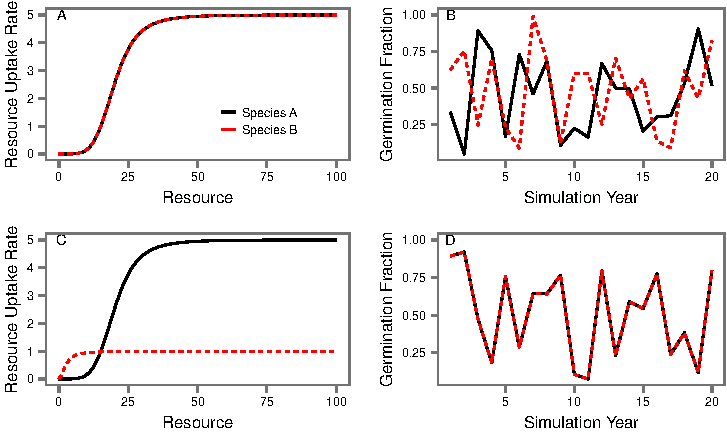
\includegraphics{components/figure/manuscript-model_types-1.pdf}
\caption{Resource uptake functions and example time series of
(un)correlated germination fractions for the storage effect (A,B) and
relative nonlinearity (C,D) formulations of the consumer-resource model.
The resource uptake functions for both species are equivalent for the
storage effect, but their germination fractions are uncorrelated in
time. The opposite is true for relative nonlinearity: the two species
have unique resource uptake functions, but their germination fractions
are perfectly correlated in time.}
\end{figure}

\newpage{}

\begin{figure}[!ht]
  \centering
      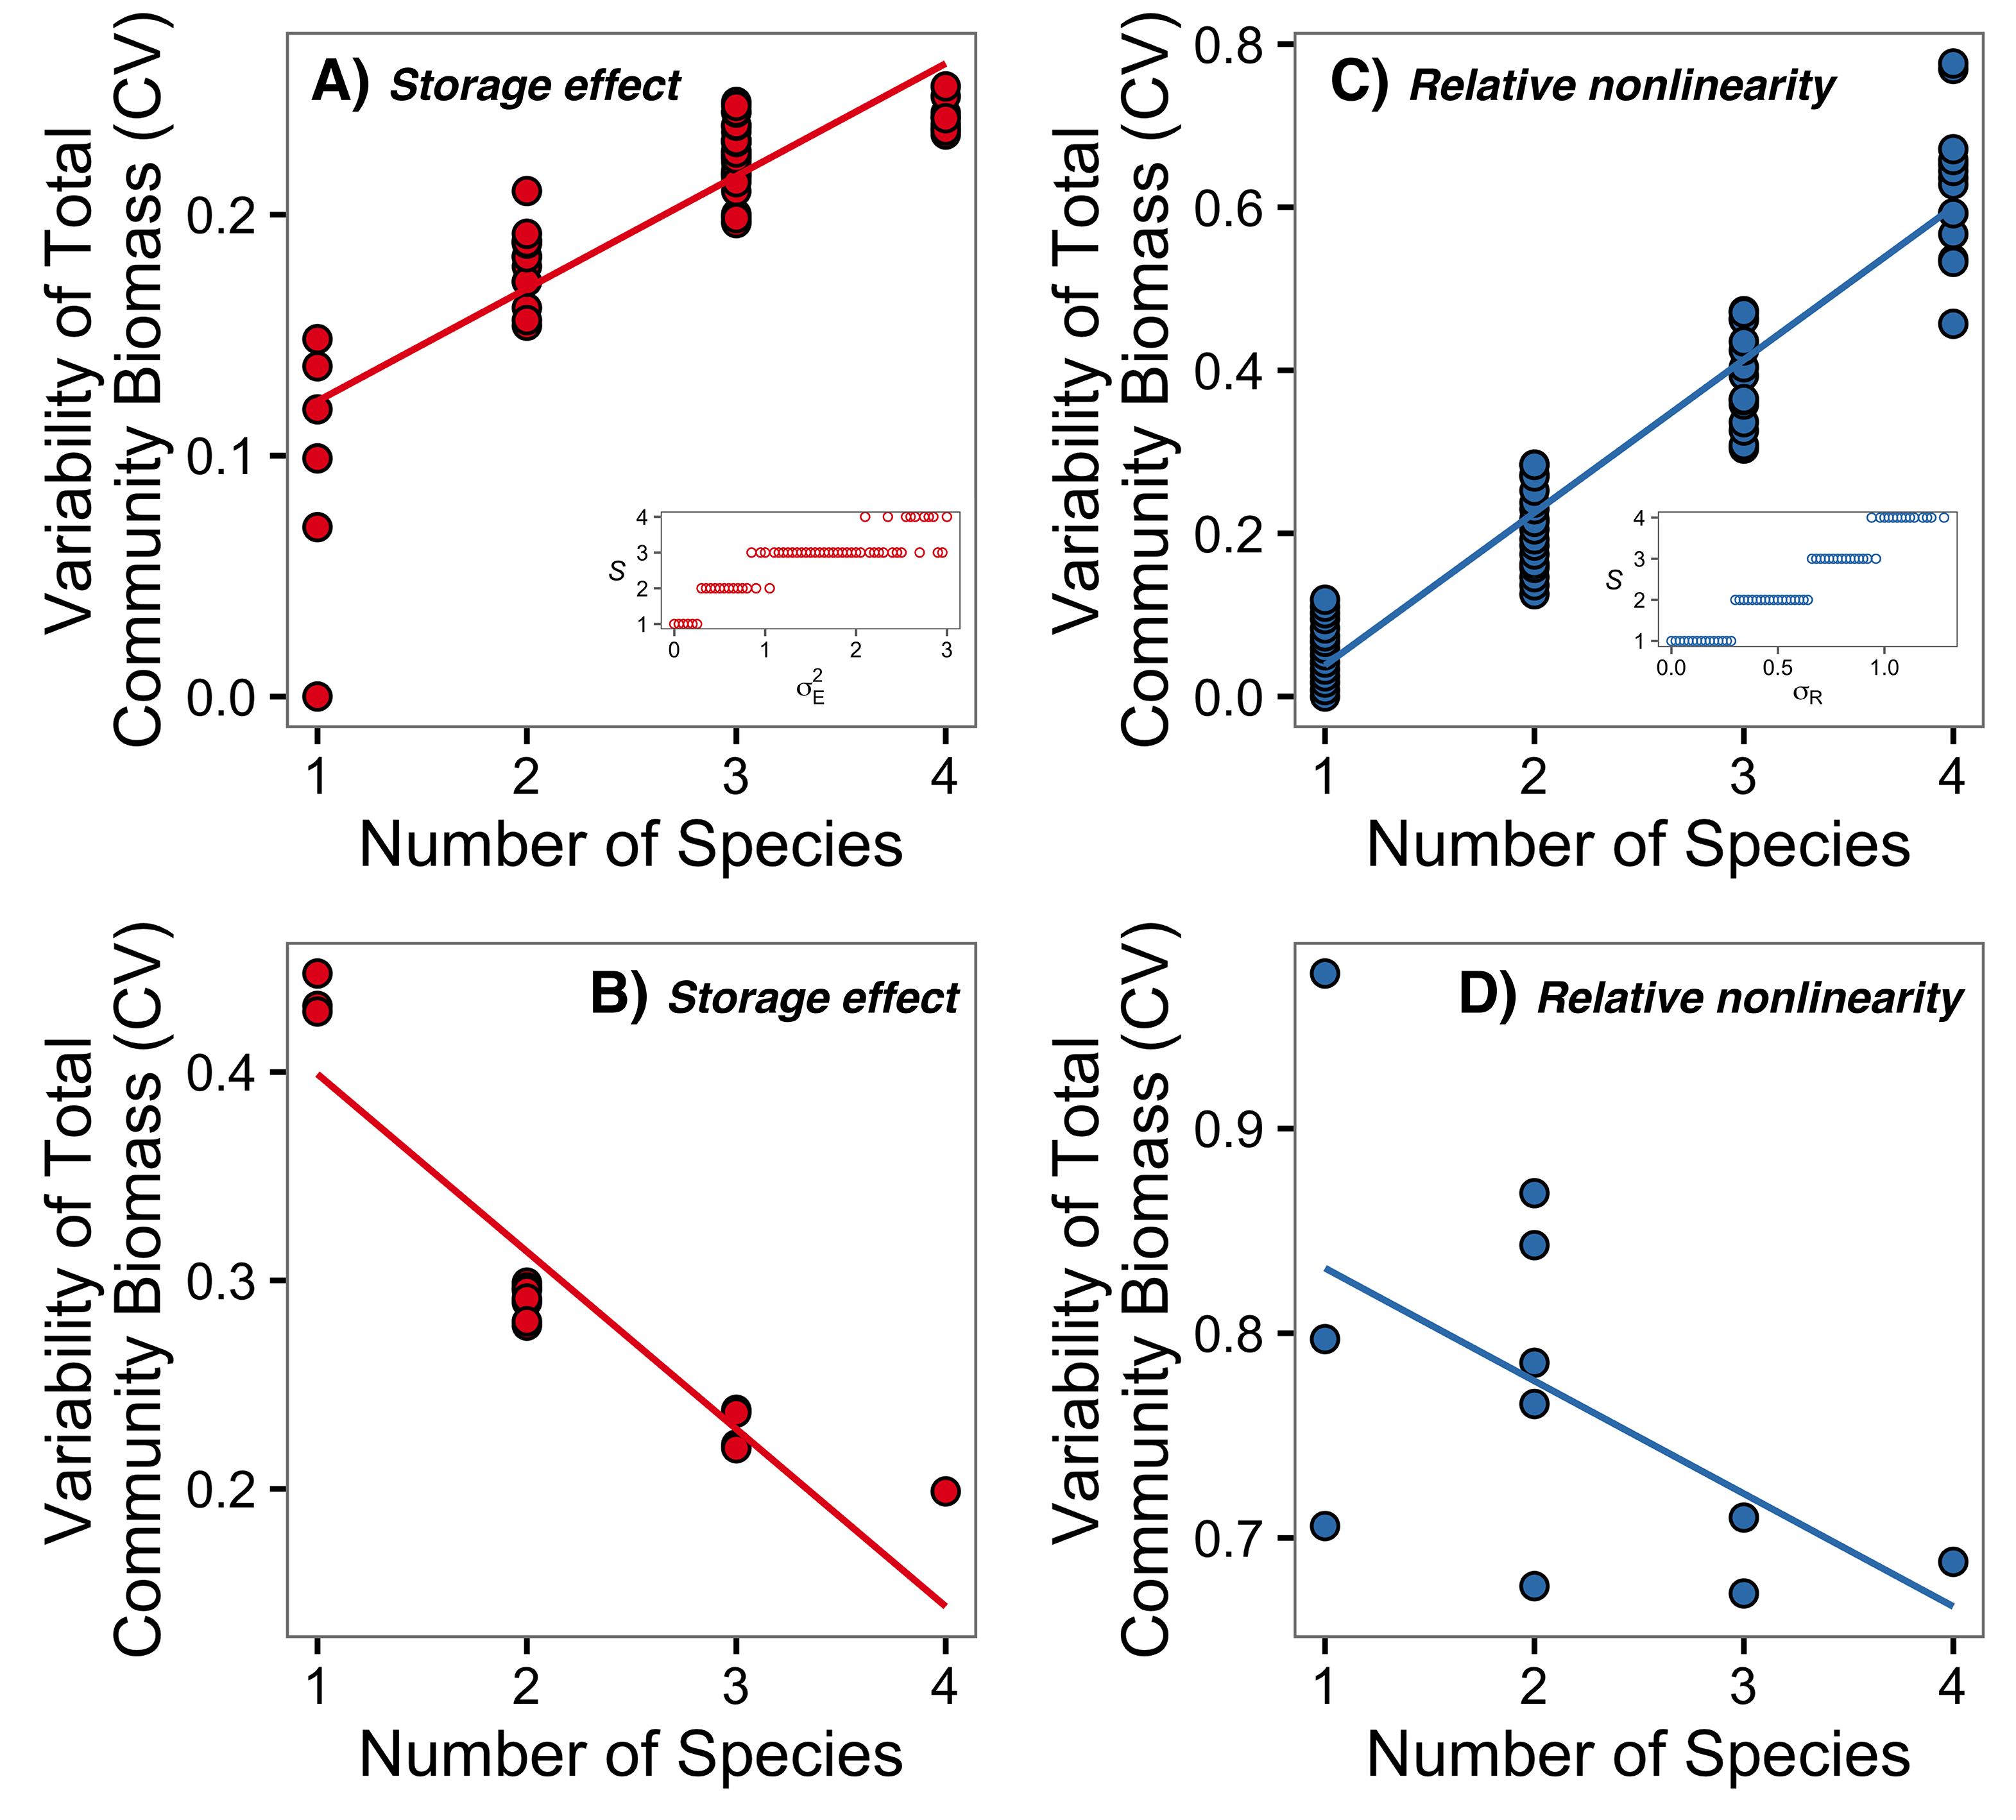
\includegraphics{./components/main_figure_hires.png}
  \caption{Variability of total community as function of species richness when coexistence is maintained by the storage effect (A,B) or relative nonlinearity (C,D). Top panels show results from simulations where environmental or resource variance determine the number species that coexist in a community. Bottom panels show results from simulations where environmental or resource variance is fixed at a level that allows coexistence of all four species, but speces are removed to manipulate diversity. The top panels represent regional diversity-stability relationships across natural diversity gradients, whereas the bottom panels represent local diversity-stability relationships.}
\end{figure}

\newpage{}

\begin{figure}[!ht]
  \centering
      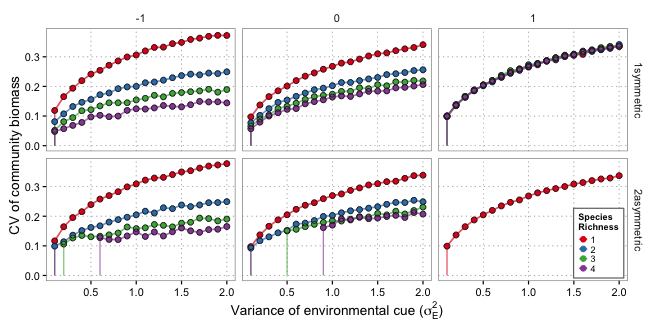
\includegraphics[height=5in]{./components/storage_effect_div+envar_varycomp.png}
  \caption{The effect of environmental variability on ecosystem variability with associated effects of species richness when species coexist via the storage effect. Panels (A-C) show simulation results where species have slightly asymmetrical competitive effects, whereas panels (D-F) show results when competition is more asymmetric. We show results for different levels of correlations of species' environmental responses, $\rho$.}
\end{figure}

\newpage{}

\begin{figure}[!ht]
  \centering
      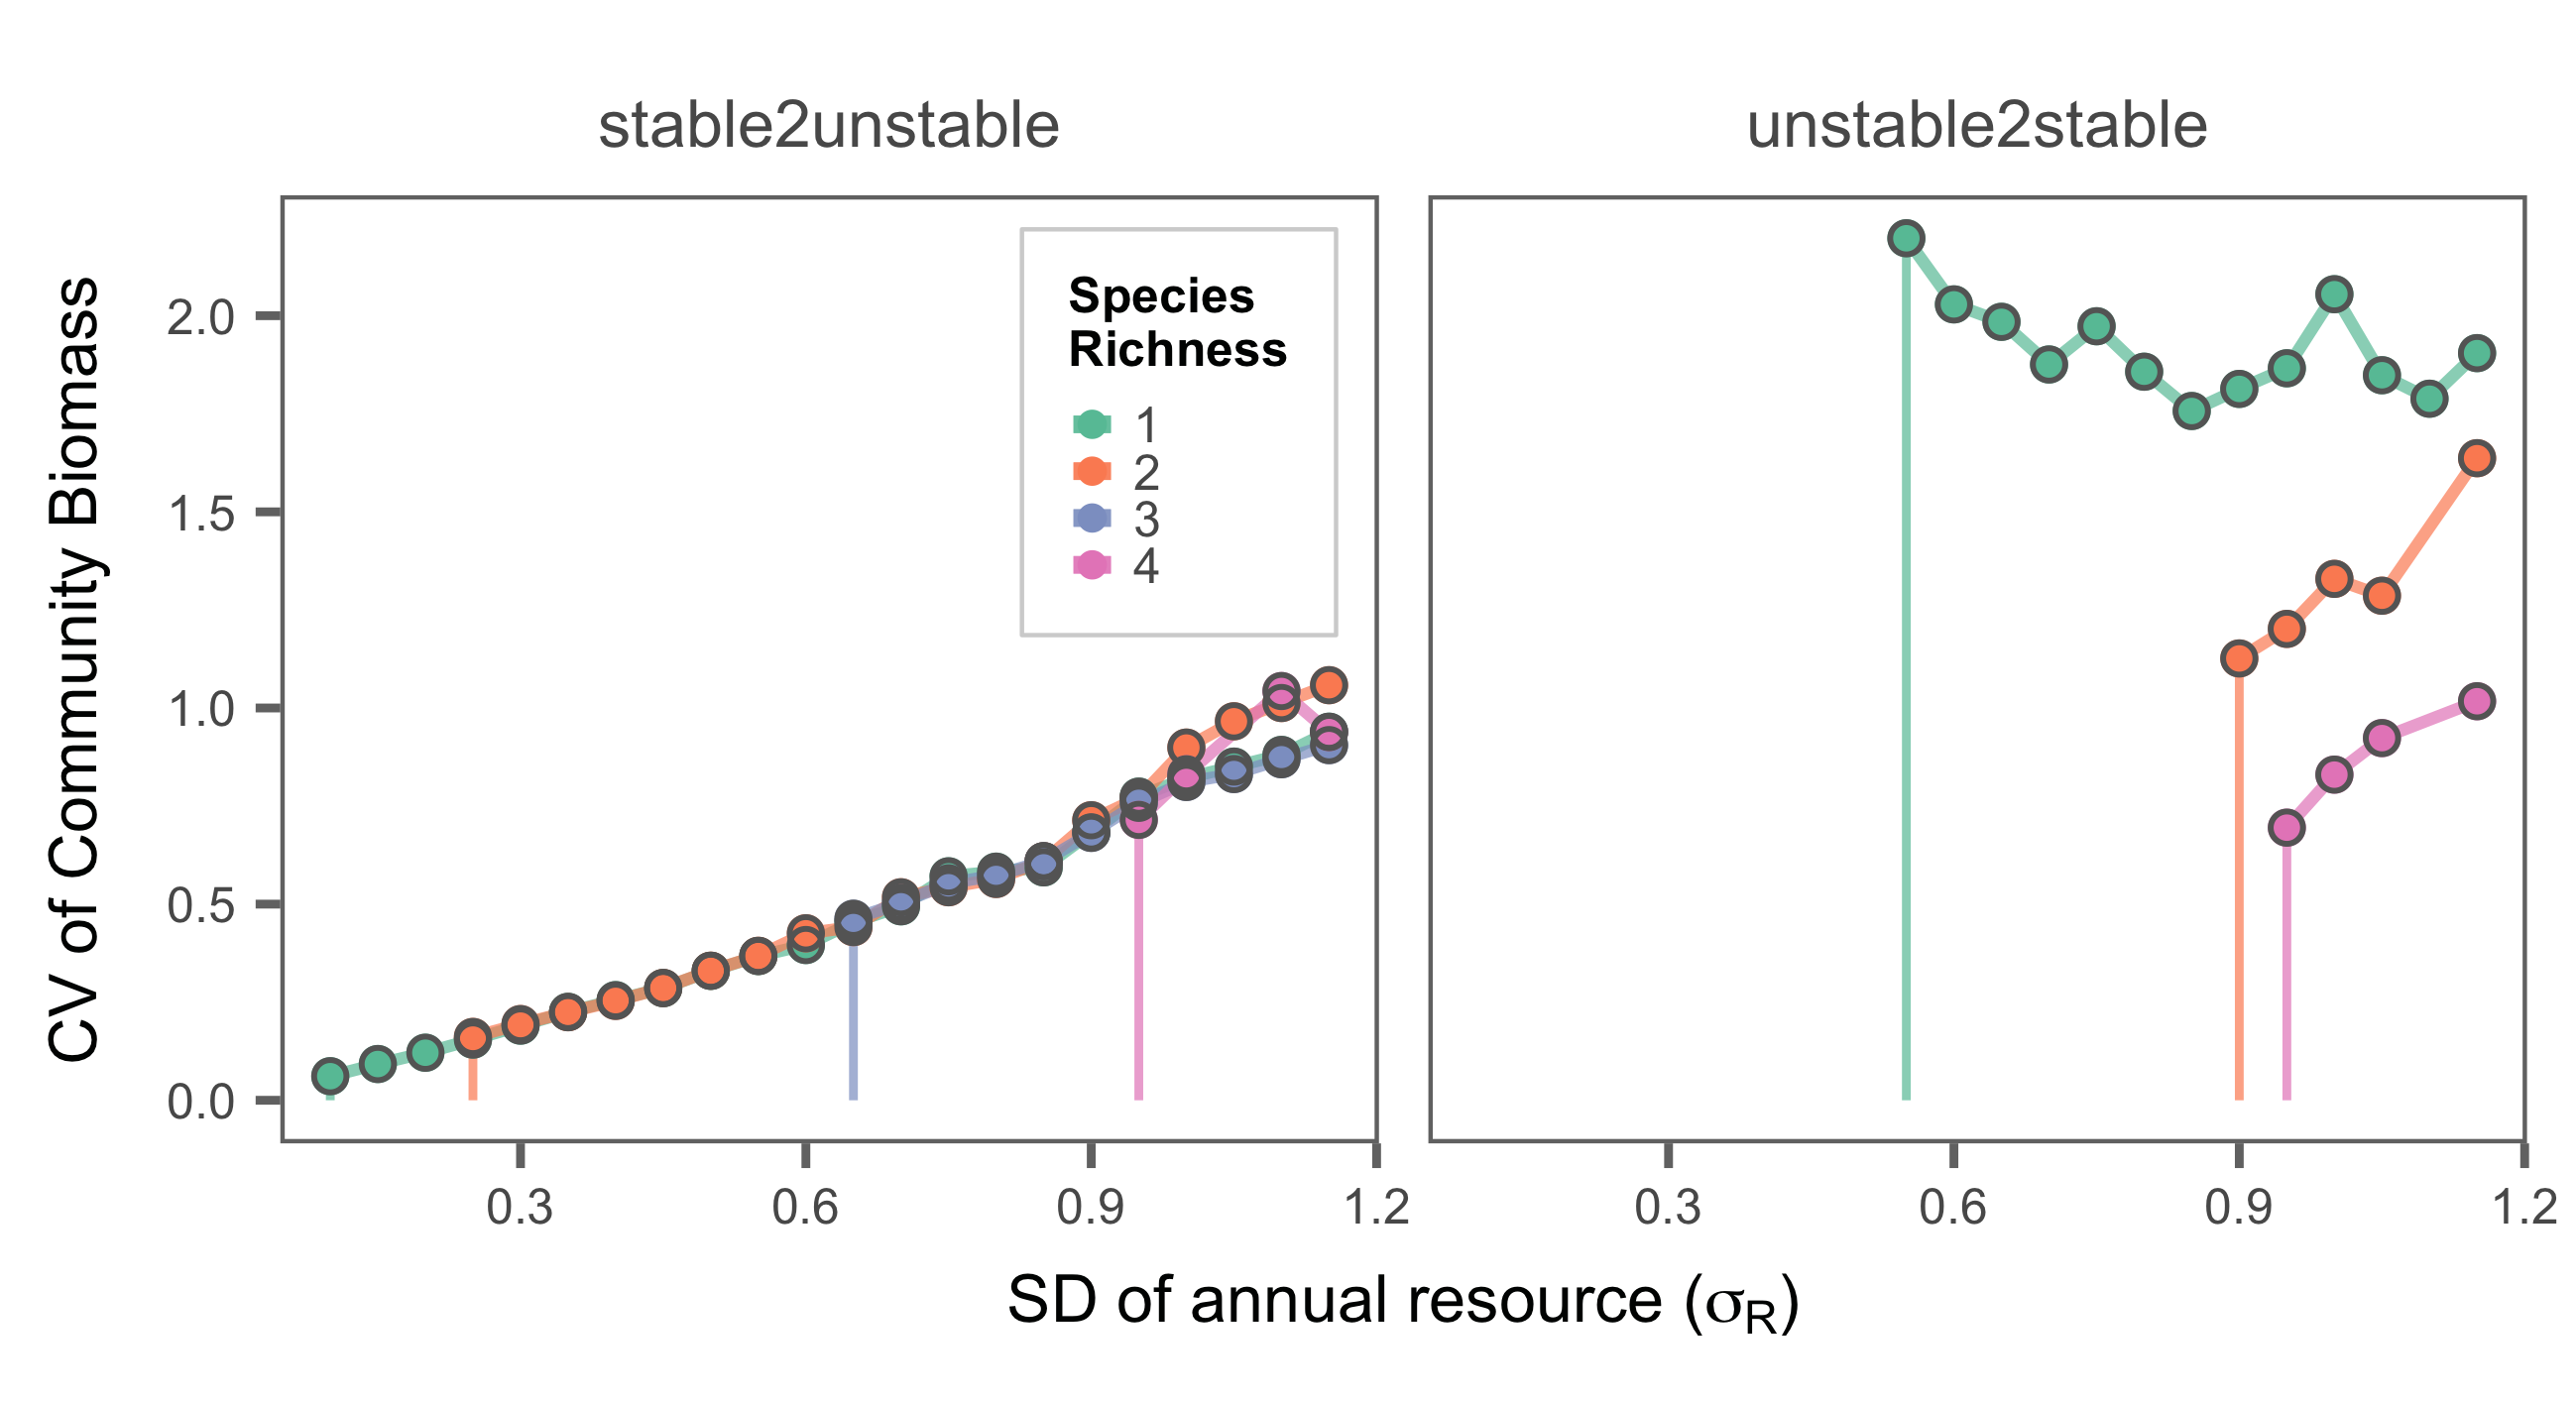
\includegraphics[height=2.5in]{./components/relative_nonlinearity_div+envar.png}
  \caption{The effect of environmental variability on ecosystem variability with associated effects of species richness when species coexist via relative nonlinearity. (A) The species pool increases from 1-4 four species, with the fourth species being most unstable. Increasing environmental variability (the SD of annual resource availability) allows for greater species richness, but species additions do not modulate the effect of environmental variability on ecosystem variability. (B) The species pool increases from 1-4 four species, with the fourth species being most stable (though, the fourth species was unable to coexist under these parameter values). In this case increasing environmental variability allows for greater realized species richness and can temper the effect of environmental variability.}
\end{figure}

\newpage{}

\begin{figure}[!ht]
  \centering
      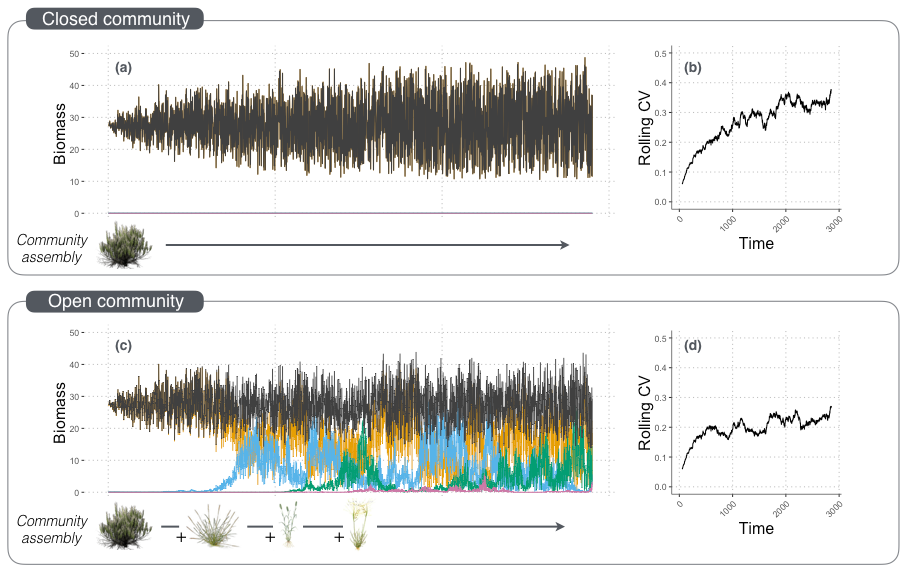
\includegraphics[height=4in]{./components/coexistence_stability_infographic_v2.png}
  \caption{Example of how species additions under increasing environmental variability can buffer ecosystem stability when species coexistence is fluctuation-dependent via the storage effect. Environmental variability ($\sigma^2_E$) increases linearly with time. (A) Time series of species' biomasses (colored lines) in a closed community where colonization of new species is not possible and (B) its associated coefficient of variation (Rolling CV; calculated over 100-yr moving window) through time. (C) Time series of species' biomasses in an open community where colonization by new species from the regional pool of four species becomes possible as environmental variation increases. The trajectory of total biomass CV in the open community (D) asymptotes at lower variability than in the closed community (B) due to the buffering effect of species richness.}
\end{figure}

\newpage{}

\setlength{\parindent}{0ex} \singlespacing

\subsection*{REFERENCES}\label{references}
\addcontentsline{toc}{subsection}{REFERENCES}

Adler, P. B., J. HilleRisLambers, P. C. Kyriakidis, Q. Guan, and J. M.
Levine. 2006. Climate variability has a stabilizing effect on the
coexistence of prairie grasses. Proceedings of the National Academy of
Sciences 103:12793--12798.

Angert, A. L., T. E. Huxman, P. Chesson, and D. L. Venable. 2009.
Functional tradeoffs determine species coexistence via the storage
effect. Proceedings of the National Academy of Sciences of the United
States of America 106:11641--11645.

Armstrong, R. A., and R. McGehee. 1980. Competitive Exclusion. The
American Naturalist 115:151--170.

Avolio, M. L., K. J. L. Pierre, G. R. Houseman, S. E. Koerner, E. Grman,
F. Isbell, D. S. Johnson, and K. R. Wilcox. 2015. A framework for
quantifying the magnitude and variability of community responses to
global change drivers. Ecosphere 6:1--14.

Brown, J. H., and A. Kodric-Brown. 1997. Turnover Rates in Insular
Biogeography : Effect of Immigration on Extinction. Ecology 58:445--449.

C{á}ceres, C. E. 1997. Temporal variation, dormancy, and coexistence: a
field test of the storage effect. Proceedings of the National Academy of
Sciences 94:9171--9175.

Chesson, P. 2000a. Mechanisms of Maintenance of Species Diversity.
Annual Review of Ecology and Systematics 31:343--366.

Chesson, P. 2000b. General theory of competitive coexistence in
spatially-varying environments. Theoretical population biology
58:211--37.

Chesson, P. L. 1994. Multispecies Competition in Variable Environments.
Theoretical Population Biology 45:227.

Chesson, P. L., and R. R. Warner. 1981. Environmental Variability
Promotes Coexistence in Lottery Competitive Systems. The American
Naturalist 117:923--943.

Chesson, P., R. L. E. Gebauer, S. Schwinning, N. Huntly, K. Wiegand, M.
S. K. Ernest, A. Sher, A. Novoplansky, and J. F. Weltzin. 2004. Resource
pulses, species interactions, and diversity maintenance in arid and
semi-arid environments. Oecologia 141:236--253.

Chesson, P., S. W. Pacala, and C. Neuhauser. 2001. Environmental Niches
and Ecosystem Functioning. Pages 213--245 \emph{in} A. P. Kinzig, S. W.
Pacala, and D. Tilman, editors. The functional consequences of
biodiversity: Empirical progress and theoretical extensions. Princeton
University Press, Princeton.

Clark, J. S., D. Bell, C. Chu, B. Courbaud, M. Dietze, M. Hersh, J.
HilleRisLambers, I. Ib{á}{ñ}ez, S. LaDeau, S. McMahon, J. Metcalf, J.
Mohan, E. Moran, L. Pangle, S. Pearson, C. Salk, Z. Shen, D. Valle, and
P. Wyckoff. 2010. High-dimensional coexistence based on individual
variation: a synthesis of evidence. Ecological Monographs 80:569--608.

Cusson, M., T. P. Crowe, R. Ara{ú}jo, F. Arenas, R. Aspden, F. Bulleri,
D. Davoult, K. Dyson, S. Fraschetti, K. Herk{ü}l, C. Hubas, S. Jenkins,
J. Kotta, P. Kraufvelin, A. Mign{é}, M. Molis, O. Mulholland, L. M.-L.
No{ë}l, D. M. Paterson, J. Saunders, P. J. Somerfield, I. Sousa-Pinto,
N. Spilmont, A. Terlizzi, and L. Benedetti-Cecchi. 2015. Relationships
between biodiversity and the stability of marine ecosystems: Comparisons
at a European scale using meta-analysis. Journal of Sea Research
98:5--14.

DeClerck, F. A. J., M. G. Barbour, and J. O. Sawyer. 2006. Species
richness and stand stability in conifer forests of the Sierra Nevada.
Ecology 87:2787--2799.

Descamps-Julien, B., and A. Gonzalez. 2005. Stable coexistence in a
fluctuating environment: An experimental demonstration. Ecology
86:2815--2824.

Eisenhauer, N., A. D. Barnes, S. Cesarz, D. Craven, O. Ferlian, F.
Gottschall, J. Hines, A. Sendek, J. Siebert, M. P. Thakur, and M.
T{ü}rke. 2016. Biodiversity-ecosystem function experiments reveal the
mechanisms underlying the consequences of biodiversity change in real
world ecosystems. Journal of Vegetation Science 27:1061--1070.

Elton, C. 1958. The Ecology of Invasions by Animals and Plants. Pages
1689--1699. University of Chicago Press, Chicago.

Hallett, L. M., J. S. Hsu, E. E. Cleland, S. L. Collins, T. L. Dickson,
E. C. Farrer, L. A. Gherardi, K. L. Gross, R. J. Hobbs, L. Turnbull, and
K. N. Suding. 2014. Biotic mechanisms of community stability shift along
a precipitation gradient. Ecology 95:1693--1700.

Harpole, W. S., L. L. Sullivan, E. M. Lind, J. Firn, P. B. Adler, E. T.
Borer, J. Chase, P. A. Fay, Y. Hautier, H. Hillebrand, A. S. MacDougall,
E. W. Seabloom, R. Williams, J. D. Bakker, M. W. Cadotte, E. J.
Chaneton, C. Chu, E. E. Cleland, C. D'Antonio, K. F. Davies, D. S.
Gruner, N. Hagenah, K. Kirkman, J. M. H. Knops, K. J. {La Pierre}, R. L.
McCulley, J. L. Moore, J. W. Morgan, S. M. Prober, A. C. Risch, M.
Schuetz, C. J. Stevens, and P. D. Wragg. 2016. Addition of multiple
limiting resources reduces grassland diversity. Nature 537:93--96.

Hautier, Y., E. W. Seabloom, E. T. Borer, P. B. Adler, W. S. Harpole, H.
Hillebrand, E. M. Lind, A. S. MacDougall, C. J. Stevens, J. D. Bakker,
Y. M. Buckley, C. Chu, S. L. Collins, P. Daleo, E. I. Damschen, K. F.
Davies, P. a Fay, J. Firn, D. S. Gruner, V. L. Jin, J. a Klein, J. M. H.
Knops, K. J. {La Pierre}, W. Li, R. L. McCulley, B. a Melbourne, J. L.
Moore, L. R. O'Halloran, S. M. Prober, A. C. Risch, M. Sankaran, M.
Schuetz, and A. Hector. 2014. Eutrophication weakens stabilizing effects
of diversity in natural grasslands. Nature 508:521--5.

Hector, A., Y. Hautier, P. Saner, L.Wacker, R. Bagchi, J. Joshi, M.
Scherer-Lorenzen, E. M. Spehn, E. Bazeley-White, M.Weilenmann, M. C.
Caldeira, P. G. Dimitrakopoulos, J. a. Finn, K. Huss-Danell, A.
Jumpponen, and M. Loreau. 2010. General stabilizing effects of plant
diversity on grassland productivity through population asynchrony and
overyielding. Ecology 91:2213--2220.

Ives, A. R., and J. B. Hughes. 2002. General relationships between
species diversity and stability in competitive systems. The American
naturalist 159:388--395.

Jiang, L., and Z. Pu. 2009. Different effects of species diversity on
temporal stability in single-trophic and multitrophic communities. The
American Naturalist 174:651--659.

Kinzig, A. P., S. W. Pacala, and D. Tilman (Eds.). 2001. The functional
consequences of biodiversity: Empirical progress and theoretical
extensions. Pages i--365. Princeton University Press, Princeton.

Klanderud, K., and Ø. Totland. 2005. Simulated climate change altered
dominance hierarchies and diversity of an alpine biodiversity hotspot.
Ecology 86:2047--2054.

Lehman, C. L., and D. Tilman. 2000. Biodiversity, Stability, and
Productivity in Competitive Communities. The American Naturalist
156:534--552.

Leibold, M. A., M. Holyoak, N. Mouquet, P. Amarasekare, J. M. Chase, M.
F. Hoopes, R. D. Holt, J. B. Shurin, R. Law, D. Tilman, M. Loreau, and
A. Gonzalez. 2004. The metacommunity concept: A framework for
multi-scale community ecology.

Loreau, M. 1998. Biodiversity and ecosystem functioning: a mechanistic
model. Proceedings of the National Academy of Sciences of the United
States of America 95:5632--5636.

Loreau, M. 2010. From Polutations to Ecosystems: Theoretical Fondations
for a New Ecological Synthesis.

Loreau, M., and C. {{de Mazancourt}}. 2013. Biodiversity and ecosystem
stability: A synthesis of underlying mechanisms. Ecology Letters
16:106--115.

MacArthur, R. 1955. Fluctuations of Animal Populations and a Measure of
Community Stability. Ecology 36:533--536.

Mailleret, L., and V. Lemesle. 2009. A note on semi-discrete modelling
in the life sciences. Philosophical transactions. Series A,
Mathematical, physical, and engineering sciences 367:4779--4799.

Mordecai, E. A., K. Gross, and C. E. Mitchell. 2016. Within-Host Niche
Differences and Fitness Trade-offs Promote Coexistence of Plant Viruses.
The American Naturalist 187:E13--E26.

Pachepsky, E., R. M. Nisbet, and W. W. Murdoch. 2008. Between discrete
and continuous: Consumer-resource dynamics with synchronized
reproduction. Ecology 89:280--288.

Sasaki, T., and W. K. Lauenroth. 2011. Dominant species, rather than
diversity, regulates temporal stability of plant communities. Oecologia
166:761--768.

Soetaert, K., T. Petzoldt, and R. W. Setzer. 2010. Package deSolve :
Solving Initial Value Differential Equations in R. Journal Of
Statistical Software 33:1--25.

Team, R. 2013. R Development Core Team. R: A Language and Environment
for Statistical Computing.

Tilman, D. 1982. Resource competition and community structure. Pages
1--296.

Tilman, D., P. B. Reich, and J. M. H. Knops. 2006. Biodiversity and
ecosystem stability in a decade-long grassland experiment. Nature
441:629--632.

Turnbull, L. A., J. M. Levine, M. Loreau, and A. Hector. 2013.
Coexistence, niches and biodiversity effects on ecosystem functioning.
Ecology Letters 16:116--127.

Valone, T. J., and C. D. Hoffman. 2003. A mechanistic examination of
diversity-stability relationships in annual plant communities. Oikos
103:519--527.

Wang, S., and M. Loreau. 2014. Ecosystem stability in space: \(\alpha\),
\(\beta\) and \(\gamma\) variability. Ecology Letters 17:891--901.

Wardle, D. A. 2016. Do experiments exploring plant diversity-ecosystem
functioning relationships inform how biodiversity loss impacts natural
ecosystems? Journal of Vegetation Science 27:646--653.

Yachi, S., and M. Loreau. 1999. Biodiversity and ecosystem productivity
in a fluctuating environment: the insurance hypothesis. Proceedings of
the National Academy of Sciences of the United States of America
96:1463--1468.

\end{document}
